\chapter{Conclusion and Final Thoughts}
\label{ch:conclusion}

\vspace{-1cm}
\begin{center}
Eduard Hirsch
\end{center}

This last chapter discusses the goals reached as well as the problems encountered during developing the INTERLACE prototype. Additionally, emphasis it put on possible enhancements necessary and issues which needs to be taken into account in order to bring that prototype to productive solution.

Finally parts are discussed which could not be finished as well as after-INTERLACE goals are addressed.

\section{Best Practices, Falsey and Pitfalls}

When using hyperledger composer but also when connecting to hyperledger fabric directly some points are important to take care of. Developers have to be aware that working with chain-code or smart contracts, although highly abstracted from the user already by various frameworks, and interacting with a distributed ledger like a blockchain, it is quite different from accessing data as usual in a RDBMS\footnote{Relational Database Management System}.

Next some of those typical peculiarities are approached and attempted to be clarified.

\subsection{Deterministic Execution}

One of the most important things to take care of when writing chain-code applications is the deterministic execution of transaction. Which seams quite obvious at the beginning is sometimes quite challenging to achieve.

One example is the \textbf{generation of IDs}:  In a standard database environment simple locking mechanisms are in place to ensure correct primary keys for entries in a table. For blockchains  which are living in a distributed, consensus-based system it is problematic to create identifiers over chain-code execution. The reason is that each peer processing a transaction would compute a new ID completely independent and most likely at the about the same time. Thus, if such a key-/ID-generation would create different IDs on different clients no consensus may be reached and although nothing is actually wrong with the transaction itself the resulting blockchain states would be different and therefore the last action would be rolled back.

This would be especially hard to deal with during race conditions and even more difficult to find out why a particular problem has been occurring.

One solution to that problem would be to generate the ID from the client and pass it to the transaction as parameter which would result in much safer creation process which is further much faster during execution.

Another problem poses the usage of \textbf{random numbers} which is fairly impossible to use in chain-code executions as such a calculation would reach obviously different results on the various peers of the network.

But also not just plain random number generation but also the \textbf{creation of a date} has a random factor. It is not possible to know when a peer in the network actually receives a new transaction and, thus, dates created during chain-code execution are different and when written into an e.g. asset also creates different blockchains on different clients and would be therefore rolled back. Even if peers would reach consensus validation of the blockchain nodes retroactively would not be possible as the date has been changed completely.

To sum up the above statements: \textbf{Chain-code needs to be executed deterministically and has to reach, given its input parameters, the same result(s) at any point in time}.

\textbf{Note:} Another consequence of that statement is that a lot of parameters can not be generated inside of chain-code but need to be provided as parameter to a transaction. But if parameters may be creatable on client-side only, it is also necessary to implement that logic in a way that these can not be used to fool the system or bring it into an inconsistent state.

\subsection{Upgrade Network}

Traditionally updating a database after changes to database model may be quite cumbersome due to new field, foreign keys and many more issues. However, for those various methods and strategies are in place for handling them.

Blockchains are usually spread over various peers storing replicated data. Therefore, in contrast to traditional databases, it is inherently more difficult to change the distributed structures to fit some new schema necessary to add a new feature or functionality.

There may be several problems updating and changing attributes and values getting it ready for the next version of the network. It is necessary to apply all changes to network before others are able to manipulate the current ledger state in order to keep consistency and reliably achieve all fixes.

Thus, it is quite important to get everything right from the beginning, as it can be extremely difficult to apply certain changes. Consequently, it is highly advisable to think about possible changes and future scenarios together with possible side-effects and costs before first deployment to production systems.

\subsection{Hyperledger Composer Specifics}

Composer can be seen as rapid-development approach and its API sits on top of hyperledger fabric framework. It tries to shield complexity from the user and aims to significantly reduce time necessary to create distributed applications for hyperledger fabric.

For INTERLACE this meant that

\begin{itemize}
	\item models could be transferred easily,
	\item chain-code could be based on those models,
	\item a REST-Server has been supplied and
	\item a web-application generator has been available.
\end{itemize}

Consequently, it is a framework ideal for prototyping. Also when finding the right cloud provider spinning up a network would be straight forward. When hosting a network without any external provider which knows how to run those networks, a lot of the initial speed during creating a network might be lost because then a much deeper understanding of the whole architecture is necessary, thus, also a higher effort is needed to get a ready implementation to work.

\textbf{Note:} For productive systems it would necessary to change to a plain fabric implementation because Composer is still in a quite early stage and there even are rumours that it will be discontinued. The reason is that some of the new features of the fabric releases are deviating from the structures implemented by composer. So it is getting more and more difficult for Hyperledger Composer developers to provide new features and functionalities available for fabric.

\section{Identity Management}
\label{sec:id-management}

Identity Management as mentioned in previous sections has been skipped for the prototype in order to simplify the environment, decrease development efforts and therefore offer an easy access to an example mutual credit system to understand the basics.

Nevertheless, it would be quickly possible to create additional participants and grant them access to the network instead of just the currently used admin-account. E.g. an identity card can be issued for the first participant defined in transaction "InitBlockchain" which is identified by "m1". The example below illustrates how that might be done:

\begin{lstlisting}[language=bash]
	composer identity issue -c admin@tutorial-network -f m1.card -u m1 -a "resource:net.sardex.interlace.Individual#m1" -x true 
\end{lstlisting}

This identity card is facilitated by the rest server and corresponds to participant in the business network. But before a user can act with that identity it is necessary when accessing the REST server to log in first and authenticate in some sort of way. To do so composer-rest-server uses an authentication middleware implemented in JavaScript called \textit{Passport.js}\footnote{\url{http://www.passportjs.org/}}.

The passport middleware offers many different authentication strategies and is a quite mature Open Source framework. An example on how to authenticate with OAuth and GitHub can be found at the Composer documentation website\footnote{\url{https://hyperledger.github.io/composer/latest/integrating/enabling-rest-authentication}} but also different schemes can be used like JSON Web Tokens (JWT\footnote{\url{https://jwt.io/}}) mentioned in the issue tracker of the Hyperledger Composer GitHub page\footnote{\url{https://github.com/hyperledger/composer/issues/2038}}.

Passport is a commonly known middleware for authentication and may be applied also for different scenarios, thus, also is usable well when swapping Composer for another technology.

\section{Future Scenarios}
\label{sec:future-scene}

Because of using hyperledger fabric it is only a matter of configuration of extending the network. The current approach taken for INTERLACE prototype, shown in figure \ref{fig:prototype-net-ext} creates a new organisation for every payment circuit dealing with their specific region. Consequently, each region would be responsible for hosting their own peers and ideally also their own certification authority (CA), however, certificates might be still handled by the Sardex CA. 

Sardex, in this scenario, is acting as a kind of knowledge provider, transferring architecture and how to run such an additional circuit getting in a similar role of a franchising cooperation. The clients and various other visible graphical interfaces may be branded in various ways, nevertheless, the underlying structure is predefined by Sardex in order to make the network work consistently.

The orderer will be handled by Sardex as well but might be later hand over to an e.g. non-profit organisation to guarantee fair and clear defined rules. To ensure a reliable system and a high performance throughput an orderer can be clustered locally but also over various regional separated areas.

\begin{figure}[htbp]
  \centering
  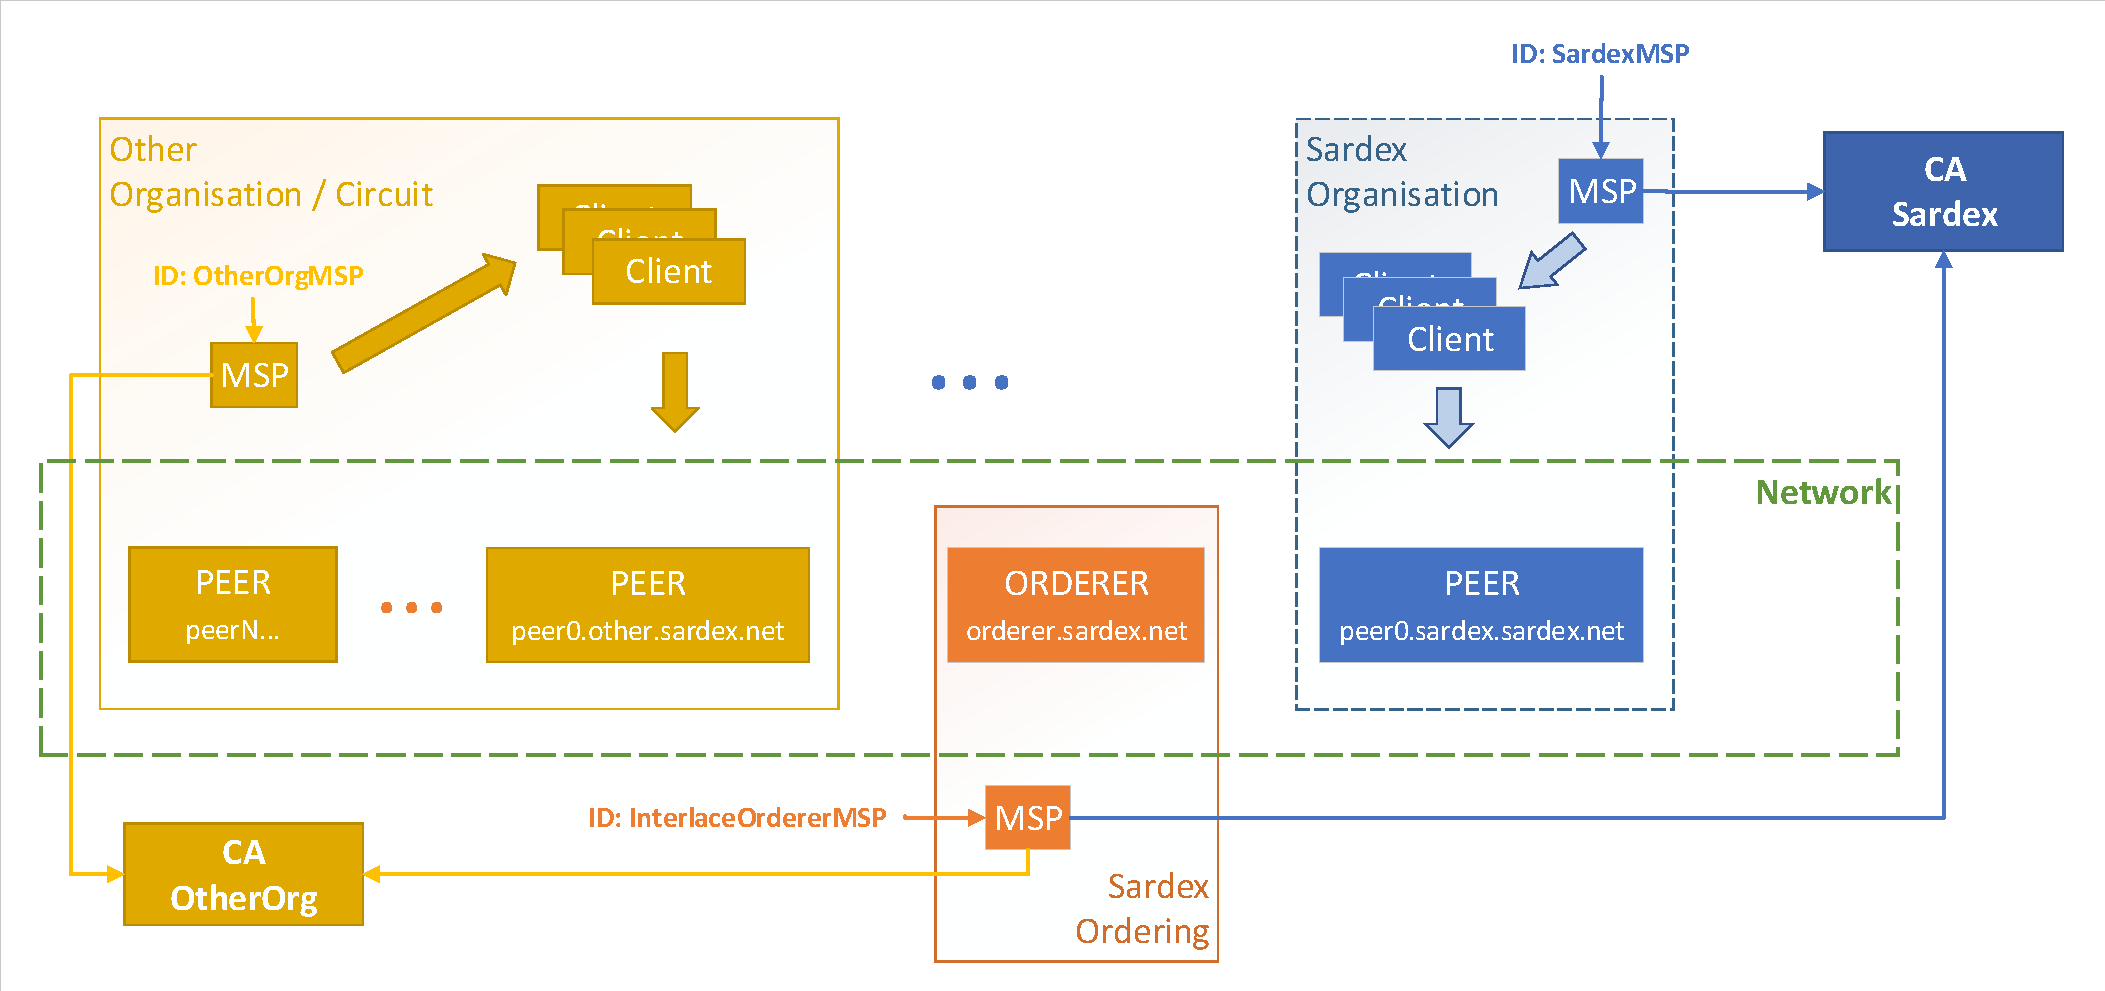
\includegraphics[width=1.0\textwidth, clip, trim=1mm 1mm 1mm 1mm]{Figures/extended-network}
  \caption{\bf\small Extended Network Structure}
  \label{fig:prototype-net-ext}
\end{figure}

\section{Final Review and Open Points}

That ledger application prototype is forming the stable and scalable basis for reliable payment circuit. Although the prototype is developed with Hyperledger Composer which IBM is pretty likely to discontinuing support for, an subsequent implementation in Hyperledger Fabric only, will be much easier to realize. Also because newer versions of fabric support an node.js SDK\footnote{Software Development Kit} which would even allow to transfer JavaScript code bits.

Basically the goal of creating a reliable DLT has been achieved and forms necessary foundation for the various other services provided in future by the productive business solution created for Sardex.

\subsection{Open Points}

The \textbf{GDPR}\footnote{General Data Protection Regulation\cite{GDPR}} taken into effect from the beginning of 2018 also posses a challenge to blockchain solutions and therefore also for the INTERLACE project. It is necessary that person related information is not exposed to other parties unless necessary and done in agreement with them. Also each information collected for and by the user needs to be deletable if requested and certainly possible to be looked up what data exactly has been collected.

Information is reliably stored inside of a blockchain, thus, looking up information is actually not an issue but rather keeping it secret from being read by other parties because standard blockchain approaches are copying everything to any peer. This is solved currently by making the actual chain only accessible by peers which are owned by the organisation running the local circuit. The Clients available for performing transfers will have restricted access an cannot see the whole blockchain.

In later stages it may be possible that every business/party participating in the payment network accessing the blockchain directly, thus, running a node. In this case the so called \textit{SideDB}\footnote{\url{https://hyperledger-fabric.readthedocs.io/en/latest/private-data/private-data.html}} is taken into consideration because it is a way offered by Hyperledger Fabric to store information which is only known by the respective client and only shared if permitted by the client.

This \textit{SideDB} also solves the problem of GDPR relevant data, because first, it is only exposed to whom it may concerned, and second, it can be purged without making the chain invalid. The reason is that in case of SideDB only hashes of transactions and data is kept inside the chain still being verifiable because of the generated hashes. Nevertheless, the data only needs to be provided if specifically asked for, e.g. in case of an (external) audit.

The second point which needs further efforts is the part of the testing coverage where the \textbf{ASIM implementations} are \textbf{tested} against the actual implementation of the prototype and later against the productive implementation. These test will be covered in deliverable 4.1 and 4.2.